\articlehead{The \adjsp My Little Pony Cocktail}{JM}{2013}

Recently I spent an afternoon watching \textit{My Little Pony: Friendship is Magic}, in an attempt to understand why ponies have become so visible in the furry community.

Criticising the show brought one expected reaction: MLP devotees thought I was unreasonably negative and dismissive of the show’s qualities. But the fact is, I had a blast: the show is charming. Plus I was drunk.

In that spirit, I am proud to present the Official [adjective][species] My Little Pony Cocktail: Vodka is Magic. (Alternate subtitle: The Party Cannon.)

\begin{wrapfigure}{l}{0.3\textwidth}
  \begin{center}
    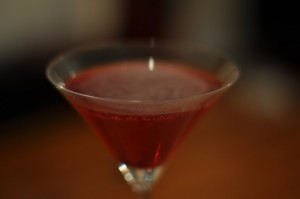
\includegraphics[width=0.25\textwidth]{content/assets/mlp--drink}
  \end{center}
  \caption{Vodka is magic.}
\end{wrapfigure}

It’s bright pink, sweet without being saccharine, and will put you at peace with the world. This recipe is enough to get one person very drunk.

\begin{itemize}
  \item 500 mL (about 15 fl oz) beetroot-infused vodka
  \item 100 mL (3 fl oz) sweet white vermouth, perhaps Martini Bianco
  \item juice and peel of 1/2 lemon
  \item 1 tablespoon sugar
\end{itemize}

Directions: Shake over lots of ice until the sugar has dissolved. Strain out the lemon peel and serve, perhaps with another block of ice. Commence \textit{MLP:FiM} viewing marathon.

\secdiv

You’ll need to make your own beetroot vodka. It’s easy, and thrifty: the infusion process will mellow cheap vodka into something perfectly drinkable.

First, cook one medium beetroot: the easiest way is to wrap a raw beetroot in aluminium foil and pop it into a moderate oven (160 $^{\circ}$C / 320 $^{\circ}$F) for an hour or two, until it’s tender (timing isn’t critical). Slip the skin off under cold running water.

You may be able to buy pre-cooked beetroot, sometimes sold in vacuum packs. Do not use pickled beetroot from a tin. That would be bad.

Slice your beetroot, add it to a bowl or a jar, and pour your vodka over the top. Cover it with an airtight lid (cling film is fine). Leave it to infuse at room temperature for a couple of days. Again, timing isn’t critical: anything from a few hours to a week will be fine.

\secdiv

Vodka is Magic will announce itself with an incongruous whiff of beetroot, and a bracingly strong first sip. From there, it’s warming and comforting.

You might serve Vodka is Magic in a martini glass, but it’s not a martini. It’s more a sister drink to the Cosmopolitan, stronger and less sour but equally appropriate for time spent in the company of pastel equines with ludicrous manes.

Happy drinking.
